\documentclass{article}

\usepackage{siunitx}
\usepackage{graphicx}
\usepackage{tikz}
\usepackage{pgfplots}

\usepgfplotslibrary{dateplot}
\usepgfplotslibrary{units}
\usetikzlibrary{external}
\tikzexternalize

\begin{document}
\tikzsetnextfilename{fig_near_ssn}
\tikzset{external/force remake}
\begin{tikzpicture}

\tikzset{
	exclude point/.style = {fill = black, opacity = 0.25, circle, scale = 0.5}
	}

\tikzset{
	proof point/.style = {fill = green, opacity = 0.75, circle, scale = 0.25}
	}

\tikzset{
	mark point/.style = {fill = violet, opacity = 0.50, circle, scale = 0.25}
	}

\node (ssn) at (0,0) {
	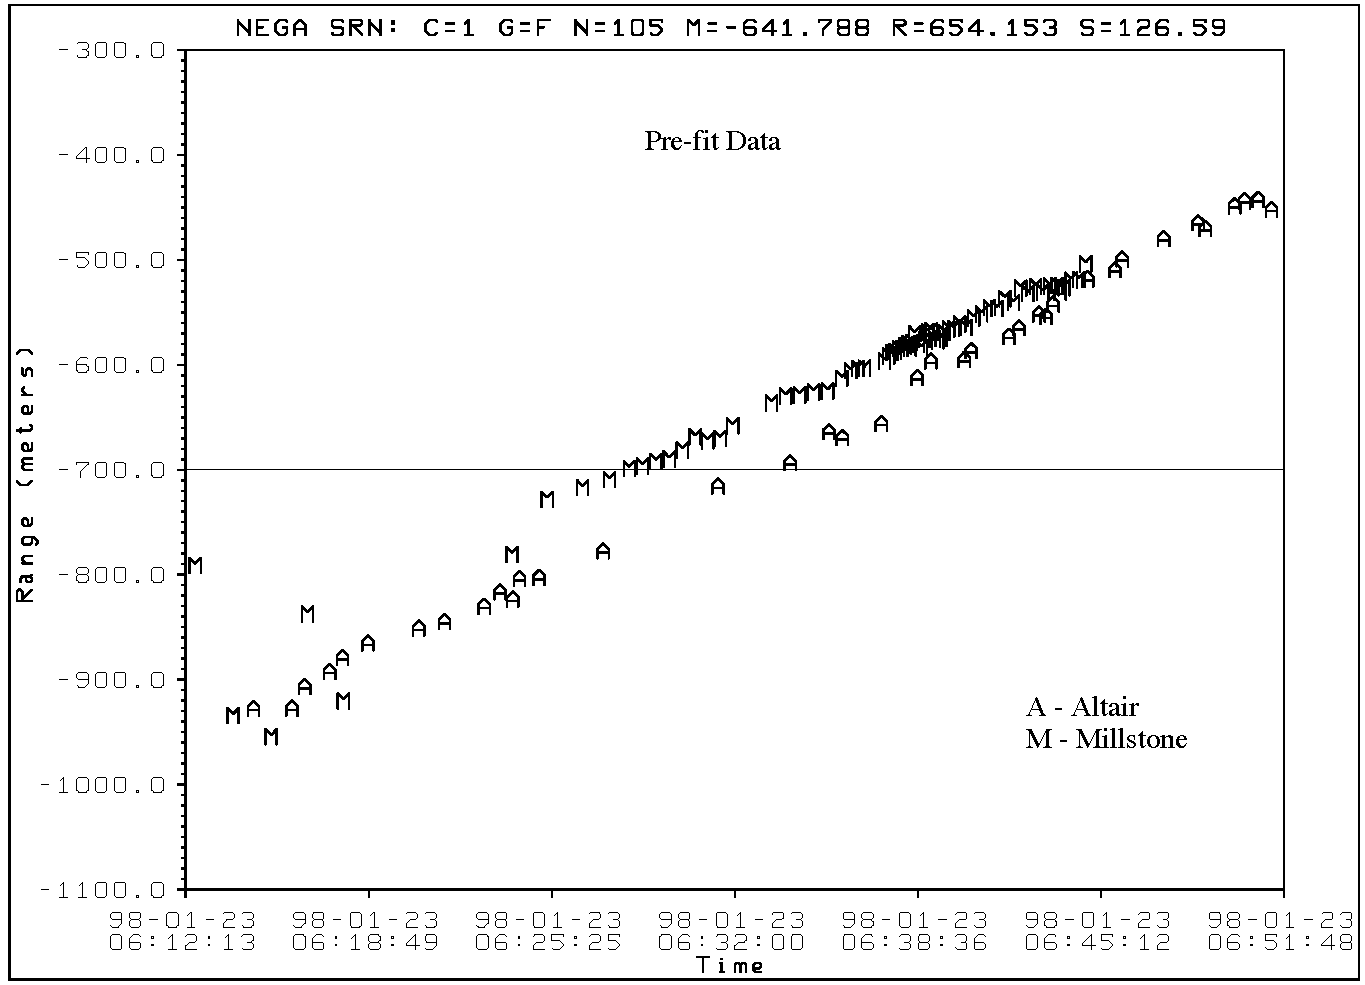
\includegraphics[width=.9\textwidth] {Antreasian/fig10_near_SSNrange.pdf}
	};

\node (jplh) at (-0.37,-0.25) {
	\begin{tikzpicture}
		[ xscale = 1.2825, yscale = 1.18 ]
	\footnotesize
	\begin{axis} [
		date coordinates in = x,
		date ZERO=1998-01-23,
		xmin={1998-01-23 06:12:00},
		xmax={1998-01-23 06:52:00},
		scaled ticks = false,
		tick align = inside,
		xtick pos = left,
		xticklabel = {\tiny \hour:\minute},
		xticklabel style = {anchor = south, color = blue},
		%
		ymax = -300,
		ymin = -1100,
		ytick pos = left,
		minor y tick num = 0,
		yticklabel = {\tiny ~\pgfmathprintnumber{\tick} \si{\metre}},
		yticklabel style = {anchor = west, color = blue},
		ylabel = {},
		%
		grid = none,
		legend style={
			at = {(0.50,0.30)},
			anchor = north,
			draw = none,
			font = \tiny,
			fill = none
			}
		]
		\draw [fill=orange!30, orange!30, opacity=0.2]
			(axis cs:1998-01-23 06:15, -300)
			--
			(axis cs:1998-01-23 06:15, -1100)
			--
			(axis cs:1998-01-23 06:12, -1100)
			--
			(axis cs:1998-01-23 06:12, -300)
			;

		\node [rotate = 90, below, orange]
			at (axis cs:1998-01-23 06:13, -700) {\tiny\it Goldstone};

		\addplot [mark = none, blue,
			y filter/.code={\pgfmathparse{\pgfmathresult-25}}
			]
			table [x index=0, y index=9, col sep=tab, skip first n=1]
			{near_altair.t};

		\addlegendentry[blue] {$\Delta r$-25 for ALTAIR (\si{\metre})};

		\addplot [mark = none, red]
			table [x index=0, y index=9, col sep=tab, skip first n=1,
				restrict y to domain=-1100:-500
			]
			{near_millstone.t};

		\addlegendentry[red] {$\Delta r$ for Millstone (\si{\metre})};

		\addplot [mark = none, blue, dotted,
			y filter/.code={\pgfmathparse{\pgfmathresult-50}}
			]
			table [x index=0, y index=9, col sep=tab, skip first n=1]
			{near_altair.t};

		\addplot [mark = none, blue, dotted]
			table [x index=0, y index=9, col sep=tab, skip first n=1]
			{near_altair.t};

		\addlegendentry[blue] {\SI{\pm 25}{\metre} bounds for ALTAIR};

		\addplot [mark = none, red, dotted,
			y filter/.code={\pgfmathparse{\pgfmathresult-5}}
			]
			table [x index=0, y index=9, col sep=tab, skip first n=1,
				restrict y to domain=-1100:-500
			]
			{near_millstone.t};

		\addplot [mark = none, red, dotted,
			y filter/.code={\pgfmathparse{\pgfmathresult+5}},
			]
			table [x index=0, y index=9, col sep=tab, skip first n=1,
				restrict y to domain=-1100:-500
			]
			{near_millstone.t};

		\addlegendentry[red] {\SI{\pm 5}{\metre} bounds for Millstone};

		% millstone
		\node [exclude point] at (axis cs:1998-01-23 06:12.40, -790) {};
		\node [exclude point] at (axis cs:1998-01-23 06:13.75, -935) {};
		\node [exclude point] at (axis cs:1998-01-23 06:15.15, -955) {};
		\node [exclude point] at (axis cs:1998-01-23 06:16.45, -838) {};
		\node [exclude point] at (axis cs:1998-01-23 06:17.75, -920) {};
		\node [exclude point] at (axis cs:1998-01-23 06:23.90, -780) {};

		\node [proof point] at (axis cs:1998-01-23 06:25.20, -730) {};
		\node [proof point] at (axis cs:1998-01-23 06:36.80, -605) {};
		\node [proof point] at (axis cs:1998-01-23 06:44.80, -505) {};

		% altair
		\node [mark point] at (axis cs:1998-01-23 06:14.50, -929) {};
		\node [mark point] at (axis cs:1998-01-23 06:15.90, -929) {};
		\node [mark point] at (axis cs:1998-01-23 06:16.34, -908) {};

		\node [mark point] at (axis cs:1998-01-23 06:17.25, -894) {};
		\node [mark point] at (axis cs:1998-01-23 06:17.75, -881) {};
		\node [mark point] at (axis cs:1998-01-23 06:18.67, -867) {};

		\node [mark point] at (axis cs:1998-01-23 06:20.50, -853) {};
		\node [mark point] at (axis cs:1998-01-23 06:21.45, -847) {};

		\node [mark point] at (axis cs:1998-01-23 06:22.90, -832) {};
		\node [mark point] at (axis cs:1998-01-23 06:23.45, -818) {};
		\node [mark point] at (axis cs:1998-01-23 06:23.94, -825) {};
		\node [mark point] at (axis cs:1998-01-23 06:24.18, -805) {};
		\node [mark point] at (axis cs:1998-01-23 06:24.90, -804) {};

		\node [mark point] at (axis cs:1998-01-23 06:27.22, -779) {};

		\node [mark point] at (axis cs:1998-01-23 06:31.40, -717) {};

		\node [mark point] at (axis cs:1998-01-23 06:34.02, -695) {};

		\node [mark point] at (axis cs:1998-01-23 06:35.42, -666) {};
		\node [mark point] at (axis cs:1998-01-23 06:35.93, -671) {};

		\node [mark point] at (axis cs:1998-01-23 06:37.36, -658) {};

		\node [mark point] at (axis cs:1998-01-23 06:38.65, -614) {};
		\node [mark point] at (axis cs:1998-01-23 06:39.15, -598) {};

		\node [mark point] at (axis cs:1998-01-23 06:40.35, -597) {};
		\node [mark point] at (axis cs:1998-01-23 06:40.64, -588) {};

		\node [mark point] at (axis cs:1998-01-23 06:42.00, -575) {};
		\node [mark point] at (axis cs:1998-01-23 06:42.35, -567) {};

		\node [mark point] at (axis cs:1998-01-23 06:43.10, -553) {};
		\node [mark point] at (axis cs:1998-01-23 06:43.35, -556) {};
		\node [mark point] at (axis cs:1998-01-23 06:43.58, -544) {};
		\node [mark point] at (axis cs:1998-01-23 06:43.85, -533) {};

		\node [mark point] at (axis cs:1998-01-23 06:44.89, -520) {};
		\node [mark point] at (axis cs:1998-01-23 06:45.85, -512) {};
		\node [mark point] at (axis cs:1998-01-23 06:46.10, -501) {};

		\node [mark point] at (axis cs:1998-01-23 06:47.63, -482) {};
		\node [mark point] at (axis cs:1998-01-23 06:48.85, -467) {};
		\node [mark point] at (axis cs:1998-01-23 06:49.15, -472) {};

		\node [mark point] at (axis cs:1998-01-23 06:50.20, -450) {};
		\node [mark point] at (axis cs:1998-01-23 06:50.58, -446) {};
		\node [mark point] at (axis cs:1998-01-23 06:51.05, -444) {};

		\node [mark point] at (axis cs:1998-01-23 06:51.54, -454) {};

	\end{axis}
	\begin{axis} [
		date coordinates in = x,
		date ZERO=1998-01-23,
		xmin={1998-01-23 06:12:00},
		xmax={1998-01-23 06:52:00},
		scaled ticks = false,
		tick align = inside,
		xtick pos = left,
		xticklabel = {\tiny \hour:\minute},
		xticklabel style = {anchor = south, color = blue},
		%
		minor y tick num = 0,
		ylabel = {},
		yticklabel = {\tiny ~\pgfmathprintnumber{\tick} \si{\kilo\metre}},
		yticklabel shift = -0.1cm,
		yticklabel style = {anchor = east, color = red},
		y filter/.code = {\pgfmathparse{1e-3*\pgfmathresult}},
		axis y line* = right,
		%
		grid = none,
		legend style={
			at = {(0.50,0.85)},
			anchor = north,
			draw = none,
			font = \tiny,
			fill = none
			}
		]

		\addplot [mark = none, dashed, blue]
			table [x index=0, y index=4, col sep=tab, skip first n=1]
			{near_altair.t};

		\addlegendentry[blue] {$r$ for ALTAIR (\si{\kilo\metre})};

		\addplot [mark = none, dashed, red]
			table [x index=0, y index=4, col sep=tab, skip first n=1]
			{near_millstone.t};

		\addlegendentry[red] {$r$ for Millstone (\si{\kilo\metre})};
	\end{axis}
	\end{tikzpicture}
	};
\end{tikzpicture}
\end{document}
